\documentclass{standalone}
\usepackage[utf8]{inputenc}
\renewcommand*\familydefault\sfdefault

\title{CIS 114 Final Project Proposal - UML Use Case Diagram}
\author{Leomar Durán}
\date{26 November 2021}

%%%%%%%%%%%%%%%%%%%%%%%%%%%%%%%%%%%%%%%%%%%%%%%%%%%%%%%%%%%%%%%
% CHANGELOG :
%     2021-11-27t03:15
%         associated user to their use cases
%
%     2021-11-27t03:08
%         add the user and first server actor
%
%     2021-11-27t01:24
%         create the package of use cases
%
%     2021-11-26t20:37
%         documented \actor[5][1]
%
%     2021-11-26t20:25
%         added ports to actor
%
%     2021-11-26t16:40
%         created actor shapes
%
%     2021-11-26t14:53
%         started with an empty node
%%%%%%%%%%%%%%%%%%%%%%%%%%%%%%%%%%%%%%%%%%%%%%%%%%%%%%%%%%%%%%%

\usepackage{tikz} % for tikzpicture
\usetikzlibrary{calc}
\usetikzlibrary{positioning}
\usetikzlibrary{matrix}
\usetikzlibrary{shapes}

% The actor shape without scope or ports
\newcommand*\unscopedactor{%
    \draw (0,22.5pt) circle (7.5pt);% head
    \draw (0,15pt) -- ++(0,-25pt) -- ++(-15pt,-20pt);% body and left leg
    \draw (-15pt,10pt) -- ++(30pt,0);% arms
    \draw (0,-10pt) -- ++(15pt,-20pt)% right leg
}%

% The actor shape including scope and ports
% @param * adds the previous 
% @param 1 scale (default 1)
% @param 2 port name prefix
% @param 3 x-shift
% @param 4 y-shift
% @param 5 extensions after the actor within scope
\makeatletter
    \newcommand*\actor{%
        \@ifstar%
            \actor@star%
            \actor@nostar%
    }%
    \newcommand*\actor@star[5][1]{%
        % coordinates stored for positioning actors
        \newdimen\xcoord
        \newdimen\ycoord
        \pgfgetlastxy\xcoord\ycoord;%
        \actor@nostar[#1]{#2}{\xcoord+#3}{\ycoord+#4}{#5}%
    }%
    \newcommand*\actor@nostar[5][1]{%
        \begin{scope}[scale=#1,xshift=#3,yshift=#4,line width=1pt]%
            \unscopedactor;%
            % create the actor ports
            \foreach \n/\x/\y in {%
                /0/0,% central port
                -north/0/30pt,%
                -west/-15pt/10pt,%
                -east/15pt/10pt,%
                -south/0/-30pt%
            }%
                \coordinate (#2\n) at (\x,\y);%
            % \foreach \n/\x/\y
            #5%
        \end{scope}%
    }%
\makeatother

\begin{document}

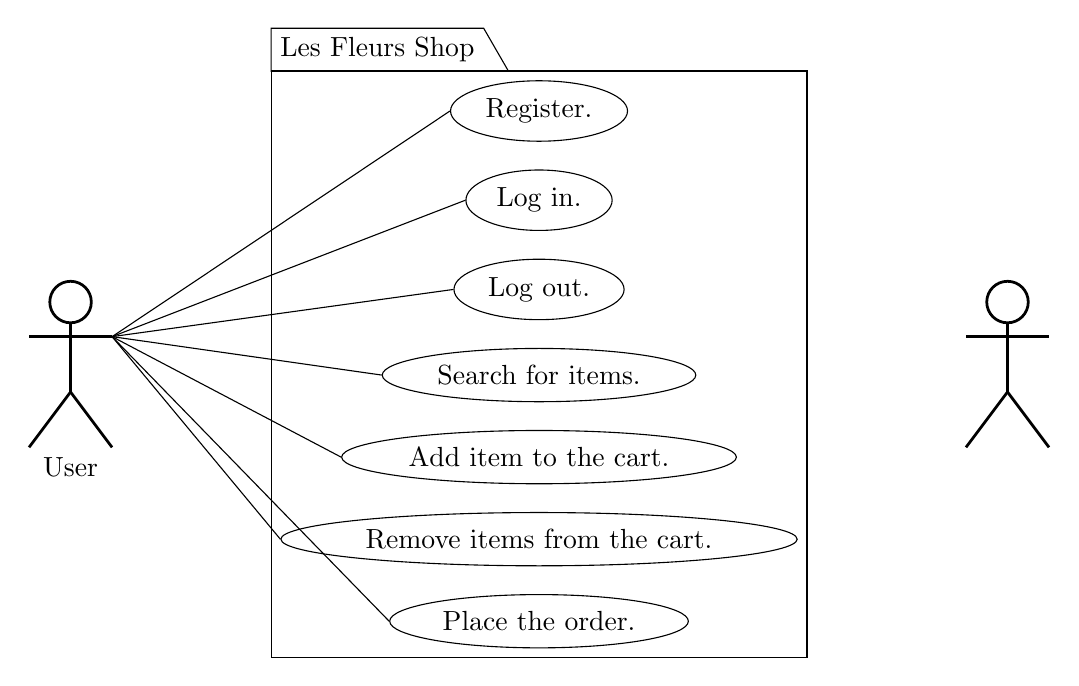
\begin{tikzpicture}
    [%
        package head/.style={%
            draw,%
            trapezium,%
            trapezium left angle=90,%
            anchor=bottom left corner,%
            yshift=-0.5pt%
        },%
        package body/.style={%
            draw,%
            matrix of nodes,%
            row sep=10pt,%
            every node/.style={use case},%
        },%
        use case/.style={%
            draw,%
            ellipse%
        }%
    ]%
%
    \matrix[package body] (les-fleurs-body) {
        Register.
    \\
        Log in.
    \\
        Log out.
    \\
        Search for items.
    \\
        Add item to the cart.
    \\
        Remove items from the cart.
    \\
        Place the order.
    \\
    };
    \node[package head] at (les-fleurs-body.north west) {Les Fleurs Shop};
%
    \node at (les-fleurs-body.west) {};
    \actor*{user}{-1in}{0pt};
    \node[below=0pt of user-south] {User};
    \foreach \k in {1,2,...,7}
        \draw (user-east) -- (les-fleurs-body-\k-1.west);
%
    \node at (les-fleurs-body.east) {};
    \actor*{server}{+1in}{0pt};
\end{tikzpicture}

\end{document}
